% PRL look and style (easy on the eyes)
\documentclass[endfloats,prl,twocolumn,superscriptaddress,nofootinbib,longbibliography]{revtex4-1}
% Two-column style (for submission/review/editing)
%\documentclass[aps,preprint,prl,superscriptaddress,showpacs]{revtex4}

\usepackage{palatino}
\usepackage{amsmath}
\usepackage{amssymb}

\usepackage{graphicx}
\usepackage{dcolumn}
\usepackage{boxedminipage}
\usepackage{verbatim}
\usepackage[colorlinks=true,citecolor=blue,linkcolor=blue]{hyperref}

\graphicspath{{figures/}}

%%% FROM NINA 

%\usepackage{fullpage}
%\usepackage{amsmath}

\newcommand{\mus}{\mu_{1 \dots n}}
\newcommand{\sigmas}{\sigma_{1 \dots n}}
\newcommand{\obsv}[1]{A_{1 \dots #1}}
\newcommand{\states}[1]{s_{1 \dots #1}}

%%%%%%%%%%% OLD STUFF (UNUSED?) %%

% italicized boldface for math (e.g. vectors)
\newcommand{\bfv}[1]{{\mbox{\boldmath{$#1$}}}}
% non-italicized boldface for math (e.g. matrices)
\newcommand{\bfm}[1]{{\bf #1}}          

%\newcommand{\bfm}[1]{{\mbox{\boldmath{$#1$}}}}
%\newcommand{\bfm}[1]{{\bf #1}}
\newcommand{\expect}[1]{\left \langle #1 \right \rangle}                % <.> for denoting expectations over realizations of an experiment or thermal averages

% vectors
%\newcommand{\x}{\bfv{x}}
%\newcommand{\y}{\bfv{y}}
%\newcommand{\f}{\bfv{f}}
%\newcommand{\z}{\bfv{z}}
%\newcommand{\p}{\bfv{p}}
%\newcommand{\q}{\bfv{q}}
%\newcommand{\T}{\mathrm{T}}

\newcommand{\op}[1]{\mathcal{#1}}
%\newcommand{\vektor}[1]{{\bf #1}}
%\renewcommand{\vec}[1]{\bfm{#1}} % italicized boldface
%\renewcommand{\vec}[1]{{\bf #1}}
\renewcommand{\vec}[1]{{\mbox{\boldmath{$#1$}}}}
\newcommand{\q}{\vec{q}} % coordinates
\newcommand{\p}{\vec{p}} % momenta
\newcommand{\z}{\vec{z}} % phase space point
\newcommand{\x}{\vec{x}} % general vector x
\newcommand{\M}{\bfm{M}} % diagonal mass matrix
\newcommand{\grad}{\nabla}
\newcommand{\timeavg}[1]{\overline{#1}}                    % time average over a trajectory

\newcommand{\bfc}{\bfm{c}}
\newcommand{\hatf}{\hat{f}}

\newcommand{\bTheta}{\bfm{\Theta}}
\newcommand{\btheta}{\bfm{\theta}}
\newcommand{\bhatf}{\bfm{\hat{f}}}
\newcommand{\Cov}[1] {\mathrm{cov}\left( #1 \right)}
\newcommand{\Ept}[1] {{\mathrm E}\left[ #1 \right]}
\newcommand{\Eptk}[2] {{\mathrm E}\left[ #2 \,|\, #1\right]}
\newcommand{\T}{\mathrm{T}}                                % T used in matrix transpose
\newcommand{\qed}{\hfill \mbox{\raggedright \rule{.07in}{.1in}}}  % QED mark
\newcommand{\var}[1]{\mathrm{var} \, #1}
\newcommand{\cov}[2]{\mathrm{cov}\left( {#1}, {#2} \right)}

%% DOCUMENT %%%%%%%%%%%%%%%%%%%%%%%%%%%%%%%%%%%%%%%%%%%%%%%%%%%%%%%%%%%%%%%%%%%%
\begin{document}

%% TITLE %%%%%%%%%%%%%%%%%%%%%%%%%%%%%%%%%%%%%%%%%%%%%%%%%%%%%%%%%%%%%%%%%%%%
\title{Supplementary Material for:\\
Bayesian hidden Markov model analysis of single-molecule force spectroscopy: Characterizing kinetics under measurement uncertainty}
%\title{Characterizing equilibrium kinetics in single-molecule force spectroscopy measurements with Bayesian hidden Markov models}
% JDC: Possible subtitle: Characterizing metastable states and transition rates under measurement uncertainty

\author{John D. Chodera}
 \thanks{Corresponding author}
% \email{jchodera@berkeley.edu}
 \affiliation{California Institute of Quantitative Biosciences (QB3), University of California, Berkeley, CA 94720, USA}

\author{Phillip Elms}
% \email{elms@berkeley.edu}
 \affiliation{California Institute of Quantitative Biosciences (QB3), University of California, Berkeley, CA 94720, USA}
 \affiliation{Biophysics Graduate Group, University of California, Berkeley, CA 94720, USA}
 \affiliation{Jason L.~Choy Laboratory of Single Molecule Biophysics, Institute for Quantitative Biosciences, University of California, Berkeley, CA 94720, USA}

\author{Frank No\'{e}}
% \email{frank.noe@fu-berlin.de}
 \affiliation{DFG Research Center Matheon, FU Berlin, Arnimallee 6, 14195 Berlin, Germany}

\author{Bettina Keller}
% \email{bettina.keller@fu-berlin.de}
 \affiliation{DFG Research Center Matheon, FU Berlin, Arnimallee 6, 14195 Berlin, Germany}

\author{Christian M. Kaiser}
% \email{cmkaiser@berkeley.edu}
 \affiliation{California Institute of Quantitative Biosciences (QB3), University of California, Berkeley, CA 94720, USA}
 \affiliation{Department of Physics, University of California, Berkeley, CA 94720, USA}

\author{Aaron Ewall-Wice}
% \email{olivercromwell@uchicago.edu}
 \affiliation{University of Chicago, IL 60637, USA}

\author{Susan Marqusee}
% \email{marqusee@berkeley.edu}
 \affiliation{California Institute of Quantitative Biosciences (QB3), University of California, Berkeley, CA 94720, USA}
 \affiliation{Department of Molecular \& Cell Biology, University of California, Berkeley, CA 94720, USA}
 \affiliation{Jason L.~Choy Laboratory of Single Molecule Biophysics, Institute for Quantitative Biosciences, University of California, Berkeley, CA 94720, USA}

\author{Carlos Bustamante}
% \email{carlos@alice.berkeley.edu}
 \affiliation{California Institute of Quantitative Biosciences (QB3), University of California, Berkeley, CA 94720, USA}
 \affiliation{Department of Molecular \& Cell Biology, University of California, Berkeley, CA 94720, USA}
 \affiliation{Jason L.~Choy Laboratory of Single Molecule Biophysics, Institute for Quantitative Biosciences, University of California, Berkeley, CA 94720, USA}
 \affiliation{Department of Physics, University of California, Berkeley, CA 94720, USA}
 \affiliation{Department of Chemistry, University of California, Berkeley, CA 94720, USA}
 \affiliation{Howard Hughes Medical Institute, University of California, Berkeley, CA 94720, USA}

\author{Nina Singhal Hinrichs}
% \email{nshinrichs@uchicago.edu}
 \affiliation{Departments of Statistics and Computer Science, University of Chicago, IL 60637, USA}

\date{\today}

%%%%%%%%%%%%%%%%%%%%%%%%%%%%%%%%%%%%%%%%%%%%%%%%%%%%%%%%%%%%%%%%%%%%%%%%%%%%%%%%%%%%%%%%%%%%%%%%%%%%%%
% ABSTRACT/pacs
%%%%%%%%%%%%%%%%%%%%%%%%%%%%%%%%%%%%%%%%%%%%%%%%%%%%%%%%%%%%%%%%%%%%%%%%%%%%%%%%%%%%%%%%%%%%%%%%%%%%%%
\begin{abstract}
\end{abstract}

\maketitle

%%%%%%%%%%%%%%%%%%%%%%%%%%%%%%%%%%%%%%%%%%%%%%%%%%%%%%%%%%%%%%%%%%%%%%%%%%%%%%%%%%%%%%%%%%%%%%%%%%%%%%
% MAKE FONT SMALLER TO MATCH JOURNAL STYLE
%%%%%%%%%%%%%%%%%%%%%%%%%%%%%%%%%%%%%%%%%%%%%%%%%%%%%%%%%%%%%%%%%%%%%%%%%%%%%%%%%%%%%%%%%%%%%%%%%%%%%%
\small

%%%%%%%%%%%%%%%%%%%%%%%%%%%%%%%%%%%%%%%%%%%%%%%%%%%%%%%%%%%%%%%%%%%%%%%%%%%%%%%%%%%%%%%%%%%%%%%%%%%%%%
% vALIDATION
%%%%%%%%%%%%%%%%%%%%%%%%%%%%%%%%%%%%%%%%%%%%%%%%%%%%%%%%%%%%%%%%%%%%%%%%%%%%%%%%%%%%%%%%%%%%%%%%%%%%%%

\section{Validation}

\begin{figure}[tbp]
\noindent
\resizebox{\columnwidth}{!}{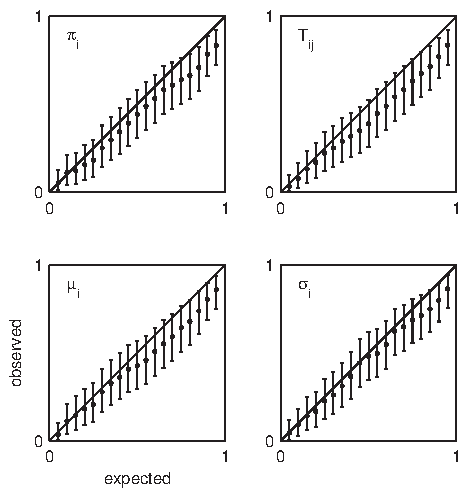
\includegraphics{confidence-intervals-random}}
\caption{{\bf Validation of confidence intervals using randomly-generated synthetic test data.}
Observed confidence intervals (points) are plotted as a function of the desired confidence intervals for equilibrium probabilities ($\pi_i$), transition probabilities ($T_{ij}$), state means ($\mu_i$), and state standard deviations ($\sigma_i$).
The black diagonal line indicates perfect agreement between expected and observed confidence intervals, while observed confidence intervals above the diagonal indicate overestimates of the uncertainty, and below the diagonal indicate underestimates.
Because only 50 random models were evaluated, error bars denote a 95\% confidence interval in the estimated observed confidence intervals.
\label{figure:validation-confidence-intervals}}
\end{figure}

The confidence interval comparison figure referred to in the main body text appears as Supplementary Figure~\ref{figure:validation-confidence-intervals}.

%%%%%%%%%%%%%%%%%%%%%%%%%%%%%%%%%%%%%%%%%%%%%%%%%%%%%%%%%%%%%%%%%%%%%%%%%%%%%%%%%%%%%%%%%%%%%%%%%%%%%%
% PROOF FOR STATE HISTORY SAMPLING
%%%%%%%%%%%%%%%%%%%%%%%%%%%%%%%%%%%%%%%%%%%%%%%%%%%%%%%%%%%%%%%%%%%%%%%%%%%%%%%%%%%%%%%%%%%%%%%%%%%%%%

\section{Proof of state history sampling scheme}
\label{section:proof-state-history-sampling}

In the reverse recursion for updating the hidden state sequence in sampling from the BHMM posterior by Gibbs sampling, we \emph{sample} a state sequence by sampling each hidden state from the conditional distribution $s_t \sim P(s_t \mid s_{t+1}, \ldots, s_L)$ starting from $t = L$ and proceeding down to $t = 0$, where the conditional distribution is given by (Eq.~35 in the main text),
\begin{eqnarray}
\lefteqn{P(s_t = i \mid s_{t+1}, \ldots, s_L)} \\
&\propto& \begin{cases}
\alpha_{t i} / \sum_{j=1}^M \alpha_{t j} & t = L \\
\alpha_{t i} T_{i s_{t+1}} / \sum_{j=1}^M \alpha_{t j} T_{j s_{t+1}} & t = (L-1),\ldots,0
\end{cases} \nonumber
\end{eqnarray} 
It is straightforward to show the result of these sampling steps reconstitutes the probability distribution $P(\bfm{S} | \bfm{T}, \bfm{E}, \bfm{O})$.
We note that the composition of these conditional distributions defines a joint distribution,
\begin{eqnarray}
\lefteqn{P(s_0 | s_1,\ldots) P(s_1 | s_2, \ldots) \cdots P(s_L) =} \nonumber \\
&=& \left[\frac{\alpha_{0 s_0} T_{s_0 s_1}}{\sum_{j=1}^M \alpha_{0 j} T_{j s_1}} \right] \left[\frac{\alpha_{1 s_1} T_{s_1 s_2}}{\sum_{j=1}^M \alpha_{1 j} T_{j s_2}} \right] \cdots \nonumber \\
&=& \left[\frac{\rho_{s_0} \varphi(o_0 | \bfm{e}_{s_0}) T_{s_0 s_1}}{\sum_{j=1}^M \alpha_{0 j} T_{j s_1}} \right] \left[\frac{\varphi(o_1 | \bfm{e}_{s_1}) \left(\sum_{j=1}^M \alpha_{0j} T_{j s_1} \right) T_{s_1 s_2}}{\sum_{j=1}^M \alpha_{1 j} T_{j s_2}} \right] \cdots \nonumber \\
&=& \frac{\rho_{s_0} \varphi(o_0 | \bfm{e}_{s_0}) T_{s_0 s_1} \cdots \varphi(o_L \mid \bfm{e}_{s_L})}{\sum_{j=1}^M \alpha_{L j}} \nonumber \\
&=& \frac{\rho_{s_0} \varphi(o_0 | \bfm{e}_{s_0}) T_{s_0 s_1} \cdots \varphi(o_L \mid \bfm{e}_{s_L})}{P(\bfm{O} | \bfm{E}) }
\end{eqnarray}
where we have used the fact that $P(\bfm{O} \mid \bfm{E}) = \sum_{j=1}^M \alpha_{tj}$,
\begin{eqnarray}
\sum_{j=1}^M \alpha_{Lj} &=& \sum_{s_L=1}^M \varphi(o_L | \bfm{e}_{s_L}) \sum_{s_{L-1}=1}^M \alpha_{(t-1) s_{L-1}} T_{s_{L-1} s_L} \nonumber \\
&=& \sum_{s_{L-1}=1}^M \alpha_{(t-1) s_{L-1}}\sum_{s_L=1}^M \varphi(o_L | \bfm{e}_{s_L})  T_{s_{L-1} s_L} \nonumber \\
%&=& \sum_{s_{L-1}=1}^M \left[ \varphi(o_{L-2} \mid \bfm{e}_{s_{L-2}}) \sum_{s_{L-2}=1}^M \alpha_{(L-2) s_{L-2}} T_{s_{L-2} s_{L-1}} \right] \sum_{s_L=1}^M \varphi(o_L | \bfm{e}_{s_L})  T_{s_{L-1} s_L} \nonumber \\
&=& \sum_{s_0} \rho_{s_0} \varphi(o_0 \mid \bfm{e}_{s_0}) T_{s_{0} s_{1}} \cdots \varphi(o_L \mid \bfm{e}_L) \nonumber \\
&=& \sum_{\bfm{S}} \rho_{s^{}_{0}} \varphi(o^{}_{0} \mid \bfm{e}_{s^{}_{0}}) \prod_{t=1}^{L^{}} T_{s^{}_{(t-1)} s^{}_{t}} \varphi(o^{}_{t} \mid \bfm{e}_{s^{}_{t}}) \nonumber \\
&=& P(\bfm{O} \mid \bfm{\Theta}) .
\end{eqnarray}
where the last step is seen by recursive substitution of the $\alpha_{tj}$.

%%%%%%%%%%%%%%%%%%%%%%%%%%%%%%%%%%%%%%%%%%%%%%%%%%%%%%%%%%%%%%%%%%%%%%%%%%%%%%%%%%%%%%%%%%%%%%%%%%%%%%
% THRESHOLD MODEL
%%%%%%%%%%%%%%%%%%%%%%%%%%%%%%%%%%%%%%%%%%%%%%%%%%%%%%%%%%%%%%%%%%%%%%%%%%%%%%%%%%%%%%%%%%%%%%%%%%%%%%

\section{Comparison with threshold model}
\label{section:model-system-segmentation}

To demonstrate that simply dividing the observable into non-overlapping regions with thresholds to define states leads to consistently biased model properties, we tested a simple segmentation scheme on the same three-state synthetic example considered in the main text.
Here, a mixture of Gaussians was first fit to the pooled observations (here, forces) according to the scheme described in \emph{Methods} to identify the peaks corresponding to each state.
%Observations were then allocated into discrete states using the crossing points between Gaussian mixture component density functions as dividing points.
A simple partition (or threshold) was assigned to the crossing point between each Gaussian probability density.
This threshold was used to determine changes between states and therefore transitions and lifetimes.
A maximum-likelihood transition matrix was then fit to the observed transition counts between states.

The result of this segmentation procedure is shown for trajectories of $10^3$ to $10^6$ observations in Figure~\ref{figure:model-segmentation-stateassignments}.
Even by eye, it is clear that there is a discrepancy between changes in state assignment color and changes in kinetic behavior.
Small conformational fluctuations that cause the force to transiently cross a threshold, but not commit to the new conformational state, result in the obsevation of spurious extra transitions.
These extra transitions will lead to an underestimate of the state self-transition probabilities and lifetimes, and convergence to incorrect model parameters.
This is confirmed by examination of the estimated model properties as a function of trajectory length in Table~\ref{table:synthetic-segmentation-model}.
Compare with Table I from the main text, where by $10^5$ observations, the estimated mean BHMM model parameters have attained relatively small error compared to the error in the segmentation model even for $10^6$ observations.

\begin{table}[tbp]
\eject
\caption{{\bf Estimated segmentation model parameters for synthetic timeseries data}}
\label{table:synthetic-segmentation-model}
\begin{tabular}{|c|c|cccc|}
\hline
property & true value & \multicolumn{4}{c|}{observation length} \\
 & & $10^3$ & $10^4$ & $10^5$ & $10^6$ \\ \hline
$\pi_{1}$ & $0.308$ & $0.214$ & $0.276$ & $0.278$ & $0.267$ \\
$\pi_{2}$ & $0.113$ & $0.155$ & $0.184$ & $0.178$ & $0.174$ \\
$\pi_{3}$ & $0.579$ & $0.632$ & $0.540$ & $0.544$ & $0.559$ \\
\hline
$T_{11}$ & $0.980$ & $0.859$ & $0.822$ & $0.828$ & $0.833$ \\
$T_{12}$ & $0.019$ & $0.125$ & $0.165$ & $0.158$ & $0.154$ \\
$T_{13}$ & $0.001$ & $0.016$ & $0.013$ & $0.014$ & $0.014$ \\
$T_{21}$ & $0.053$ & $0.173$ & $0.247$ & $0.246$ & $0.236$ \\
$T_{22}$ & $0.900$ & $0.523$ & $0.579$ & $0.564$ & $0.577$ \\
$T_{23}$ & $0.050$ & $0.304$ & $0.174$ & $0.190$ & $0.187$ \\
$T_{31}$ & $0.001$ & $0.005$ & $0.007$ & $0.007$ & $0.006$ \\
$T_{32}$ & $0.009$ & $0.074$ & $0.059$ & $0.062$ & $0.058$ \\
$T_{33}$ & $0.990$ & $0.920$ & $0.934$ & $0.930$ & $0.935$ \\
\hline
$\mu_{1}$ & $3.000$ & $2.707$ & $2.716$ & $2.746$ & $2.737$ \\
$\mu_{2}$ & $4.700$ & $4.841$ & $4.707$ & $4.714$ & $4.710$ \\
$\mu_{3}$ & $5.600$ & $5.636$ & $5.621$ & $5.619$ & $5.618$ \\
\hline
$\sigma_{1}$ & $1.000$ & $0.842$ & $0.804$ & $0.806$ & $0.806$ \\
$\sigma_{2}$ & $0.300$ & $0.330$ & $0.332$ & $0.339$ & $0.334$ \\
$\sigma_{3}$ & $0.200$ & $0.201$ & $0.187$ & $0.182$ & $0.183$ \\
\hline
\end{tabular}
\end{table}

\begin{figure*}[p]
\noindent
\resizebox{\textwidth}{!}{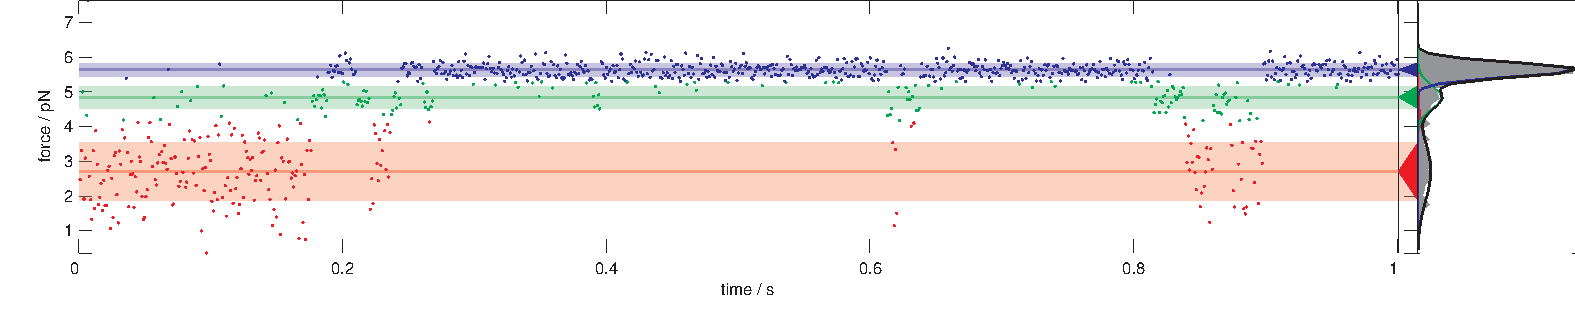
\includegraphics{model-segmentation-stateassignments-1000}}
\resizebox{\textwidth}{!}{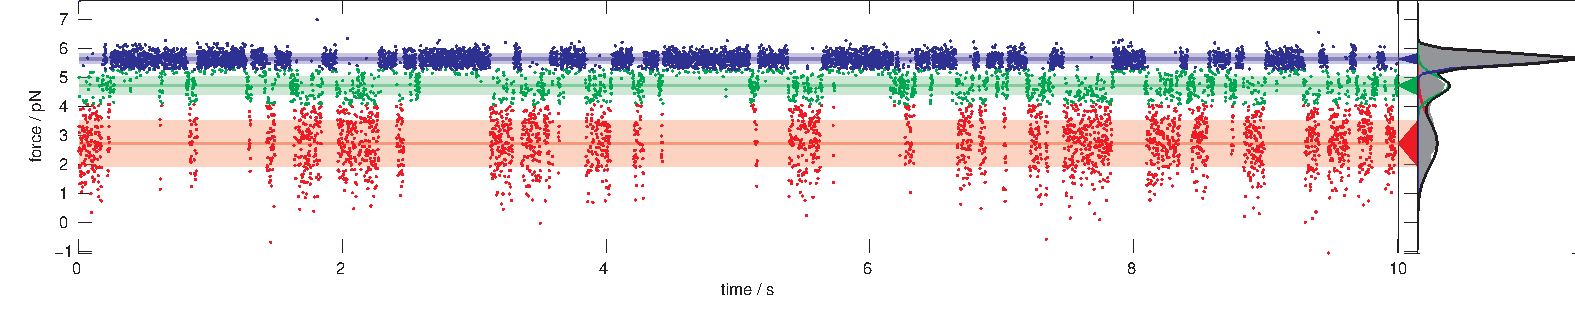
\includegraphics{model-segmentation-stateassignments-10000}}
\resizebox{\textwidth}{!}{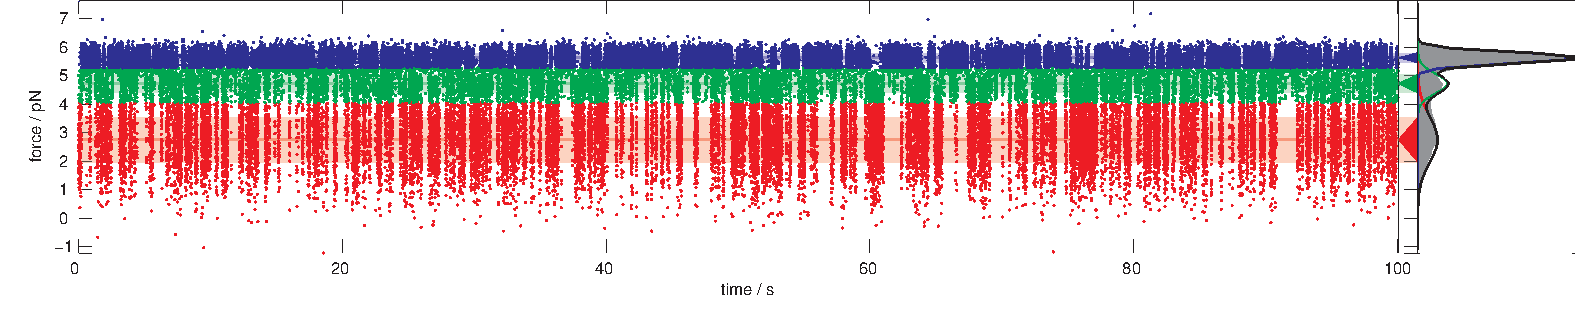
\includegraphics{model-segmentation-stateassignments-100000}}
\resizebox{\textwidth}{!}{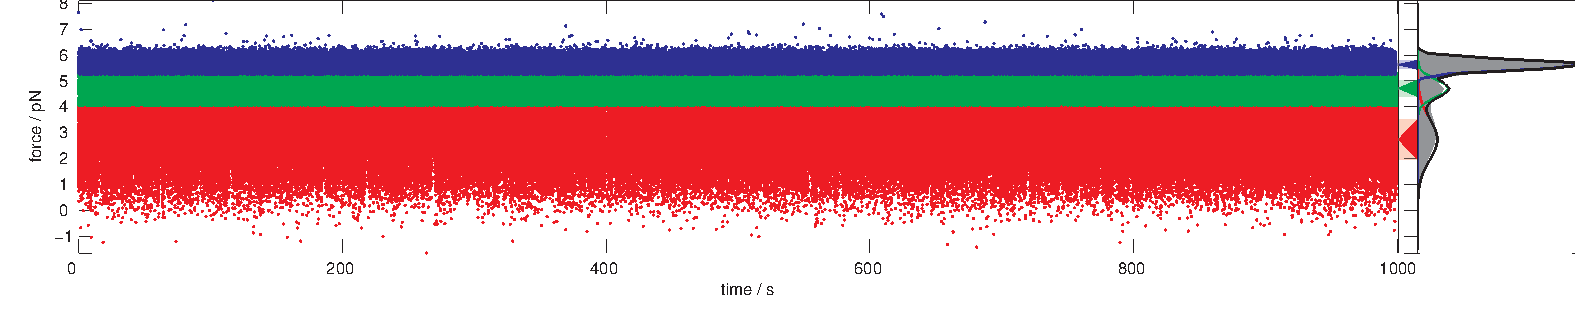
\includegraphics{model-segmentation-stateassignments-1000000}}
\caption{{\bf Synthetic force trajectory and segmentation state assignments.}
Observed samples are colored by their hidden state assignments from a model in which the observable is segmented into regions that correspond to each state, for trajectories of length $10^3$ (\emph{top}), $10^4$ (\emph{upper middle}), $10^5$ (\emph{lower middle}), and $10^6$ (\emph{bottom}) observations.
The segmentation was derived by first fitting the set of all observed forces to a mixture of Gaussians and then dividing the observations at the crossing points of the Gaussian mixture component probability density functions.
Dark horizontal lines terminating in triangles to the right denote state means, while lightly colored bands indicate one standard deviation on either side of the state mean.
The gray histogram on the right side shows the total observed probability of samples, while the colored peaks show the contribution from each state, assuming a Gaussian fit to the mean and standard deviation.
\label{figure:model-segmentation-stateassignments}}
\end{figure*}

%%%%%%%%%%%%%%%%%%%%%%%%%%%%%%%%%%%%%%%%%%%%%%%%%%%%%%%%%%%%%%%%%%%%%%%%%%%%%%%%%%%%%%%%%%%%%%%%%%%%%%
% CORRELATION FUNCTIONS
%%%%%%%%%%%%%%%%%%%%%%%%%%%%%%%%%%%%%%%%%%%%%%%%%%%%%%%%%%%%%%%%%%%%%%%%%%%%%%%%%%%%%%%%%%%%%%%%%%%%%%

\section{Choice of observation interval for hairpin}
\label{section:choice-of-markov-time}

To determine that a 1 ms time was an appropriately Markovian time for the observation interval $\Delta t$ used in HMM analysis, the autocorrelation function of the experimental force trace was computed at the full 50 kHz time resolution for a trap position where only a single conformational state appeared to dominate (Figure~\ref{figure:p5ab-autocorrelation}).
An initial nonexponential or multiexponential (with unclear number of components) decay is seen within the first 0.5 ms to approximately one tenth of the initial value, with slow decay following.
We therefore chose a 1 ms time resolution as appropriate for describing the slow conformational dynamics between states.

\begin{figure}[p]
\noindent
\resizebox{\columnwidth}{!}{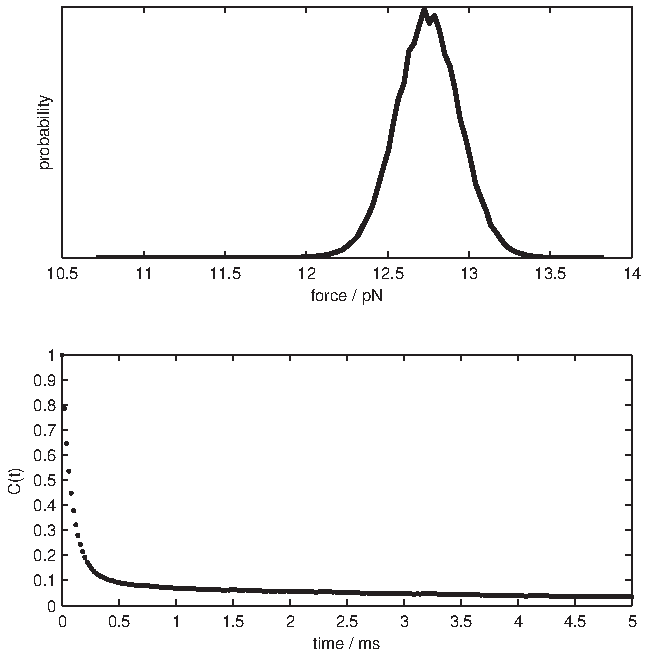
\includegraphics{fiber3-trace14-autocorrelation}}
\caption{{\bf Normalized fluctuation autocorrelation function for p5ab hairpin under conditions stabilizing a single conformation.}
\emph{Top:} The force histogram for a trap position (different from that in main text Fig.~4) showing that a single conformational state is dominant at this trap configuration.
\emph{Bottom:} The normalized integrated autocorrelation function for the force trace, showing rapid decay of non-Markovian contributions within 1 ms.
\label{figure:p5ab-autocorrelation}}
\end{figure}

\widetext
\eject

\end{document}
